\PassOptionsToPackage{utf8}{inputenc}
\documentclass{bioinfo}
\copyrightyear{2020} \pubyear{2020}
\newcommand{\R}{\mathbb{R}}
\usepackage{amsmath}
\DeclareMathOperator*{\argmax}{argmax}
\access{Advance Access Publication Date: Day Month Year}
\appnotes{ISMB 2020}
\begin{document}
\firstpage{1}

\subtitle{Subject Section}

\title[short Title]{
CoRAE: Concreate Relaxation Autoencoder for Differentiable Gene Selection and Pan-Cancer Classification
% Pan-Cancer Feature Selection and Classification Reveals Key RNAs for Cancers
% Epigenetic Landscape Using Pan-Cancer Feature Selection and Classification
}
\author[Sample \textit{et~al}.]{Abdullah Al Mamun\, and Ananda Mondal}
% $^{\text{\sfb 1,}*}$, Co-Author\,$^{\text{\sfb 2}}$ and Co-Author\,$^{\text{\sfb 2,}*}$}

\address
{
% $^{\text{\sf 1}}$
School of Computing and Information Sciences, Miami, US \\
% $^{\text{\sf 2}}$
% Department, Institution, City, Post Code,Country.
}

\corresp{$^\ast$To whom correspondence should be addressed.}

\history{Received on XXXXX; revised on XXXXX; accepted on XXXXX}

\editor{Associate Editor: XXXXXXX}

\abstract{\textbf{Motivation:} Selecting relevant features from a high-dimensional dataset is a critical study. It aims to select a small subset of features that will increase accuracy and decrease the cost of data classification or clustering. Due to high-dimension with a low number of samples in omics data, classification models encounter over-fitting problem. Therefore, there is a demand for efficient feature selection methods that will be capable of selecting relevant features. 
In recent years, standard autoencoder and its variations have been used to select latent features to increase the classification performance. However, these methods are unable to provide which original features are contributing to these latent features. In this paper, we introduced a novel global feature selection method based on concrete relaxation discrete random variable selection,  which can efficiently identify a subset of most significant features that have an effective contribution in data reconstruction and classification. The proposed method is a variation of standard autoencoder where a concrete feature selection layer is added in the encoder and a standard neural network is used as a decoder. During training, a predefined temperature of the feature selection layer steadily decreased which allows the model to learn a user-specified number of discrete features. Also, during testing, only selected features can be used to reconstruct the input in the decoder.\\
\textbf{Results:} We evaluated the proposed feature selection method on coding and non-coding gene expression of 33 cancer samples from TCGA where it significantly outperforms state-of-the-art methods in identifying top 100 coding and non-coding genes. Later, expression of selected genes is used to train a linear classifier to dishtinghish 33 cnacer types where features selected by CoRAE shows highest performance up to $99\%$. The proposed method can be implemented by adding a few lines of code to the standard autoencoder.\\\\
\textbf{Availability:} Source code and sample dataset can be found in https://github.com/pwaabdullah/MyPhD.git\\
\textbf{Contact:} \href{amondal@fiu.edu}{amondal@fiu.edu}\\
\textbf{Supplementary information:} Supplementary data are available at \textit{Bioinformatics}
online.}

\maketitle

\section{Introduction} \label{intro}
The well-known issue of recent omics data is a feature-sample ratio which is highly imbalanced means the number of features is way more than the number of samples. Among all the available features, few might be meaningful for distinguishing the samples which belong to different classes and the rest of these are either irrelevant, redundant, or noise \citep{pirgazi2019efficient}. During classification or clustering the high dimensional data, irrelevant features cause unnecessary computational complexities and decrease the performance. Therefore, it is essential to identify the most relevant features that would have a high contribution to the classificaiton or clustering of the data. During the feature selection process, redundant features are removed because there is a subset of features that carries approximate similar information. In a similar fashion, noise features that provide no information about labels are also be removed from the database. Thus, only relevant features will be remain that will increase the efficiency of any classification or clustering problems \citep{liu2012feature}. 
Any dataset with $N$ number of features has $2^N$ possible subset of features. The goal of feature selection algorithms is to find the most precise subset of features. Due to having a large number of possible combinations, finding the best subset of N features is computationally challenging and costly \cite{liang2018review}.

Filter, wrapper, embedded are the types of feature selection methods. Numerous algorithms have been proposed for each type of feature selection method. 
In the filtering method, a rank is assigned to each feature depending on the statistical relevance to the class type. In both univariate and multivariate filter method, feature-feature interactions are not considered in the selection process. Some example studies such as Pearson correlation coefficient(PC), t-statistics(TS) \citep{speed2003statistical}, F-Test \citepp{ding2005minimum}, and ANOVA \citep{ding2015identification}. These methods are effective for selecting features for high-dimensional data because of its fewer computation expenses but failed to provide a good accuracy \citep{sun2018cross}. 
To enhance the performance, the wrapper method is proposed with a learning algorithm and a classifier to find a suitable subset of features. First, it generates a random solution, then it maximize an objective function using a black-box optimization method \citepp{rau2019exploring} such as Simulated Annealing \citep{jeong2018feature}, Particle Swarm Optimization \citep{xue2012particle}, Genetic Algorithm \citep{wu2011feature}, and Ant Colony Optimization \citep{kabir2012new}. Since these methods evaluate every candidate subset of feature iteratively, they can find a strong relationship between features but it increases computational expenses. 
Similarly, embedded method do so efficiently as it is a part of its learning phase. Thus, it reduces the computational costs. Some well-known example studies are  LASSO \citep{tibshirani1996regression}, recursive feature ellimation with state vector machien estimator (SVM-RFE) \citep{abdullah2019, guyon2002gene, fang2019tightly}, random forest \citep{pouyan2018random, ram2017classification}, Adabost \citep{wang2012adaboost}, KNN \citep{le2019statistical}, and autoencoder \citep{lu2019autoencoder}.

In general, feature selection methods are useful to get insight about large and complex dataset which can simplify the learning process of any machine learning algorithm. The use of feature selection is worthy when using the whole set of features is difficult to collect or costly to execute. For example, the gene expression dataset contains more than 60 thousand features with a very low number of samples. It is normal to ask: \textit{Is it possible to identify important genes those expressions can classify available disease or cancer type?} The domain of feature selection is way more dissimilar than standard dimension reduction techniques such as principal component analysis (PCA) \citep{hotelling1933analysis}, and autoencoders \citep{hinton2006reducing}. They can preserve maximum variance with a fewer number of features, however, these methods do not provide the original features of the dataset. Thus, it is impossible to eliminate redundant or irrelevant features from the dataset. 

In this paper, a novel feature subset selection method that increases the power deep autoencoder for differentiable feature selection is proposed. Our method CoRAE introduces a new layer in the autoencoder called concrete distribution of features which allows the model to select a user-defined number of original features. Idea of concrete distribution is adapted from \citep{maddison2016concrete, kingma2013auto}, and reparameterization technique to minimize the loss and reconstruction error from \citep{abid2019concrete}. 
We have tested our end-to-end model on coding and non-coding gene expression dataset and it outperforms state-of-the-art feature selection techniques. 

\begin{table*}[hbt]
\processtable{ \textbf{Sample Distribution for 33 cancers along with 75-25 split for training and testing.}  \label{Tab:01}} {\begin{tabular}{@{}llllll|llllll@{}}\toprule Sl	&	Cancer site name	&	Acronym	&	\#Sample	&	\#Train	&	\#Test	&	Sl	&	Cancer site name	&	Acronym	&	\#Sample	&	\#Train	&	\#Test\\\midrule

1	&	Adrenocortical Cancer	&	ACC	&	77	&	57	&	20	&	18	&	Lung Squamous Cell Carcinoma	&	LUSC	&	498	&	373	&	125	\\
2	&	Bladder Cancer	&	BLCA	&	407	&	305	&	102	&	19	&	Mesothelioma	&	MESO	&	86	&	64	&	22	\\
3	&	Breast Cancer	&	BRCA	&	1089	&	816	&	273	&	20	&	Ovarian Cancer	&	OV	&	375	&	281	&	94	\\
4	&	Cervical Cancer	&	CESC	&	304	&	228	&	76	&	21	&	Pancreatic Cancer	&	PAAD	&	177	&	132	&	45	\\
5	&	Bile Duct Cancer	&	CHOL	&	36	&	27	&	9	&	22	&	Pheochromocytoma \& Paraganglioma	&	PCPG	&	177	&	132	&	45	\\
6	&	Colon Cancer	&	COAD	&	301	&	225	&	76	&	23	&	Prostate Cancer	&	PRAD	&	493	&	369	&	124	\\
7	&	Large B-cell Lymphoma	&	DLBC	&	47	&	35	&	12	&	24	&	Rectal Cancer	&	READ	&	95	&	71	&	24	\\
8	&	Esophageal Cancer	&	ESCA	&	161	&	120	&	41	&	25	&	Sarcoma	&	SARC	&	258	&	193	&	65	\\
9	&	Glioblastoma	&	GBM	&	158	&	118	&	40	&	26	&	Melanoma	&	SKCM	&	465	&	348	&	117	\\
10	&	Head and Neck Cancer	&	HNSC	&	499	&	374	&	125	&	27	&	Stomach Cancer	&	STAD	&	378	&	283	&	95	\\
11	&	Kidney Chromophobe	&	KICH	&	66	&	49	&	17	&	28	&	Testicular Cancer	&	TGCT	&	132	&	99	&	33	\\
12	&	Kidney Clear Cell Carcinoma	&	KIRC	&	527	&	395	&	132	&	29	&	Thyroid Cancer	&	THCA	&	501	&	375	&	126	\\
13	&	Kidney Papillary Cell Carcinoma	&	KIRP	&	287	&	215	&	72	&	30	&	Thymoma	&	THYM	&	118	&	88	&	30	\\
14	&	Acute Myeloid Leukemia	&	LAML	&	147	&	110	&	37	&	31	&	Endometrioid Cancer	&	UCEC	&	184	&	138	&	46	\\
15	&	Lower Grade Glioma	&	LGG	&	507	&	380	&	127	&	32	&	Uterine Carcinosarcoma	&	UCS	&	56	&	42	&	14	\\
16	&	Liver Cancer	&	LIHC	&	369	&	276	&	93	&	33	&	Ocular melanomas	&	UVM	&	79	&	59	&	20	\\
17	&	Lung Adenocarcinoma	&	LUAD	&	512	&	384	&	128	&		&	Total	&		&	9566	&	7161	&	2405\\\botrule
\end{tabular}}{}
\end{table*}


\section{Materials and Methods}
\subsection{Coding and Non-coding Gene Expression}
To validated the proposed idea, TCGA RNAseq cancer (n=9566) and clinical samples for 33 cancers were downloaded from UCSC Xena database (https://xenabrowser.net). TCGA processed raw RNAseq data using Illumina HiSeq 2000 RNA sequencing platform where per-gene normalized abundance estimation were calculated with FPKM method. RNASeq normalized counts were then log transformed after adding a constant of 1. Later UCSC re-processed using GENCODE v23 transcript annotation to quantify protein coding() and non-coding transcripts() expression \citep{harrow2006gencode}. Coding genes refers to mRNA whereas non-coding genes refers to long non-coding RNA (lncRNA) in this experiment. To improve the focus on individual feature selection, we separated mRNA and lncRNA expression from combined database using TANRIC \citep{li2015tanric} provided standard list of lncRNAs. Another important reason of performing experiment on individual RNA types is because their expression level is different. The number of mRNA and lncRNA are 18731, 12309 respectively. We merged all the cancer samples for individual RNA types for further experiment. Each row is mapped to a unique Ensemble ID, and each column mapped to a patient ID. Normal patients or RNA with missing data were removed from the original dataset. Each RNA expression was further processed using min-max normalization method to achieve good training performance. 

\subsection{Concrete Relaxation Autoencoder} \label{CoRAE}
The concrete relaxation autoencoder CoRAE is a variation of original autoencoder AE \citep{hinton2006reducing} for dimension reduction. It is a neural network consists of two parts: an encoder that selects latent features and a decoder that uses selected features to reconstruct the output similar to the input. Instead of using a sequence of fully connected layers in the encoder,  we propose a concrete relaxation based feature selection layer where user can define the number of nodes (feature), $k$. This layer selects probabilistic linear arrangement of input features during training, which converge to a discrete set of $k$ features by the end of training and during the testing. 

The original features are selected based on the temperature of this layer which is tunned using an annealing schedule. More specifically, the concrete selector layer identifies $k$ number of important features as the temperature decreases to zero. For reconstructing the input, a simple decoder similar to the standard AE is used. This simple neural network can be updated based on the characteristics of the data and its complexity.
% ------read

Layer that selects the features shown in Figure \ref{fig:architecture} is called concrete variable selctor layer adpoted from concrete distribution \citepp{maddison2016concrete} and categorical represntation \citep{jang2016categorical}. Since, backpropagation does not allow computation of the parameters' gradient through stochastic nodes of standard autoencoder, gumbel $softmax$ distribution $g$ \citep{gumbel1954statistical} is a right choice to pick samples $z$ from categorical distribution with class probabilities $\alpha_k$. 

\begin{equation}
	z = \textbf{one-hot} \, (\argmax_k \, [g_k + log \, \alpha_k])
\end{equation}

Because $\argmax$ is not differentiable, simple $softmax$ function can be used as a continuous approximation of $\argmax$. The aim of using Concrete random variables is to relax the state of a discrete variable and the ralaxation degree is controlled by a temparature parameter $\tau \in (0, \infty)$. To sample a concrete random variable in $z$ dimensions with prarameter $\alpha \in \R ^z>0$ and $\tau$, one must samples a $z$-dimensional vector of $i.i.d.$ (independent and identically distributed) samples from a Gumbel distribution, $g.$ Then each element of the sample $f$ from the Concrete distribution can be defined as:

\begin{equation}
    f_k = \frac{exp((log \alpha_k + g_k)/\tau)}{\sum_{i=1} ^z exp((log \alpha_i + g_i)/T) } \; for \; k = 1,.....,z
\end{equation}

where $f_k$ refers to the $k_{th}$ element in a particular sample
vector. With the limit $\tau \to 0$, the concrete variable uniformly progresses the discrete distribution, producing one-hot vector with $f_k = 1$ with a probabilistic chance of $\alpha _k/\sum_p \alpha _p$.
The advantage of using a concrete random discrete variable is that it is differentiable $w.r.t$ $\alpha$ using reparameterization technique as mentioned by \citep{kingma2013auto}.

\begin{figure*}[hbt]
    \centering
    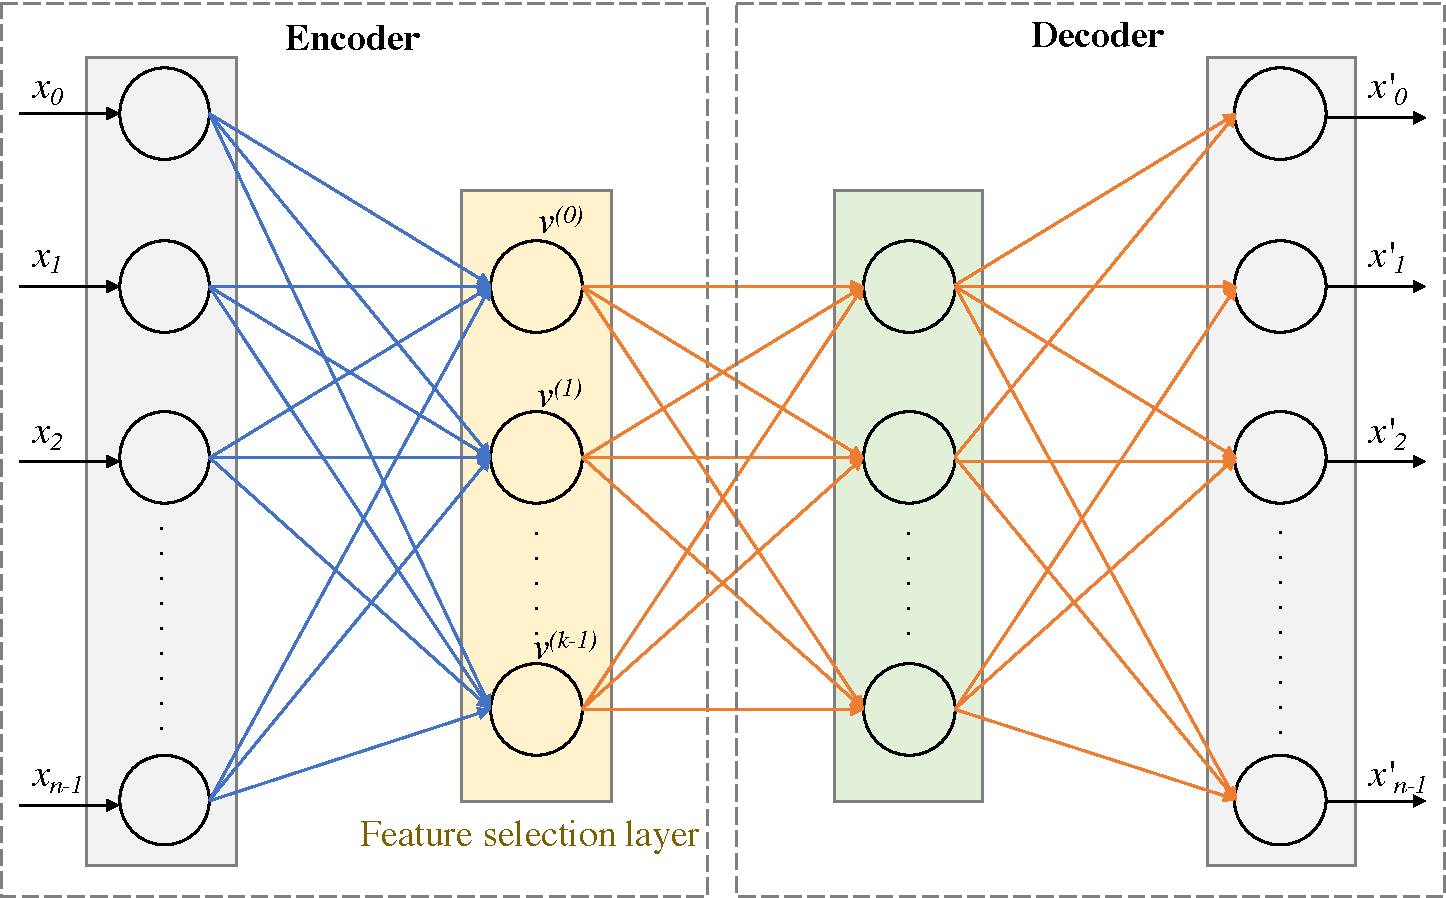
\includegraphics[scale=0.5]{fig/architecture.pdf}
    \caption{\textbf{Architecture of Concrete Relaxation Autoencoder.} Proposed feature selection architecture consists of an encoder and a decoder. The layer after input layer in encoder is called concrete feature selection layer shown in yellow. This layer has $k$ number of node where each node is for each feature to be selected. During the training stage, the $i^{th}$ node $v^{(i)}$ takes the value $x^Tf^{(i)}$.
During testing stage, these weights are fixed and the element with the highest value is selected by the corresponding $i^{th}$ hidde
n node.
The architecture of the decoder remains the same during train and test stage.}
    \label{fig:architecture}
\end{figure*}


More concisely, the way original feature is selected using the concrete random variable as follows: a $z$-dimensional concrete random variable $f^{(i)}$ is sampled for each node of the selector layer with $k$ nodes where $i$ refers to the index of the node, $i \in \{1...k\}$. The output of the $i^{th}$ node is $ \textbf{x}.f^{(i)}$. Although it is a combination of the input feature's weight, every node of the selector layer produces exactly one of the original input features in the limit $\tau \to 0$. After training the network, a discrete $\argmax$ layer is replaced with the concrete selector layer by which $x_{\argmax_j \; \alpha_j^{(i)}$ is produced as an output of $i^{th}$ node during the testing phase. The value of $\alpha_i$ initially starts with a small positive random number so that it can explore various combinations of input features. As the model is being trained, the value of $\alpha_i$, in other words the probability of class $i$ becomes more stable. As a result, the model reduces its stochasticity rather increases the confidence in drawing a particular subset of features. 

%new figure about temp

% \subsection{Annealing Schedule}

The temperature of the random variable in the selector layer has a significant impact in forming the output of each node. Initially, when $\tau$ is high, search space is large since it consideres linear combination of all features. In contrast, the selector layer will not be able to search all possible combinations of features in low $\tau$ and thus, model converges to a bad local minima. Instead of using a fixed temperature, a simple annealing scheduling scheme is used for every concrete variable. It starts with an user-defined high temperature ($\tau_s$) and steadily lessening the temperature until it touches the ending bound ($\tau_e$) by every epoch as follows: 
\begin{equation}
\tau(e) = \tau_s(\tau_N/\tau_s)^{e/N}
\end{equation}
where $T_{(e)}$ is the temperature at epoch $e$, $N$ refers to the total number of epochs. The proposed annealing schedule is good enough to explore the feature combinations during the training phase and finally lowered temperature enables the model to strict to the best set of features which is shown in Figure \ref{fig:temp}.

\begin{figure}[hbt]
    \centering
    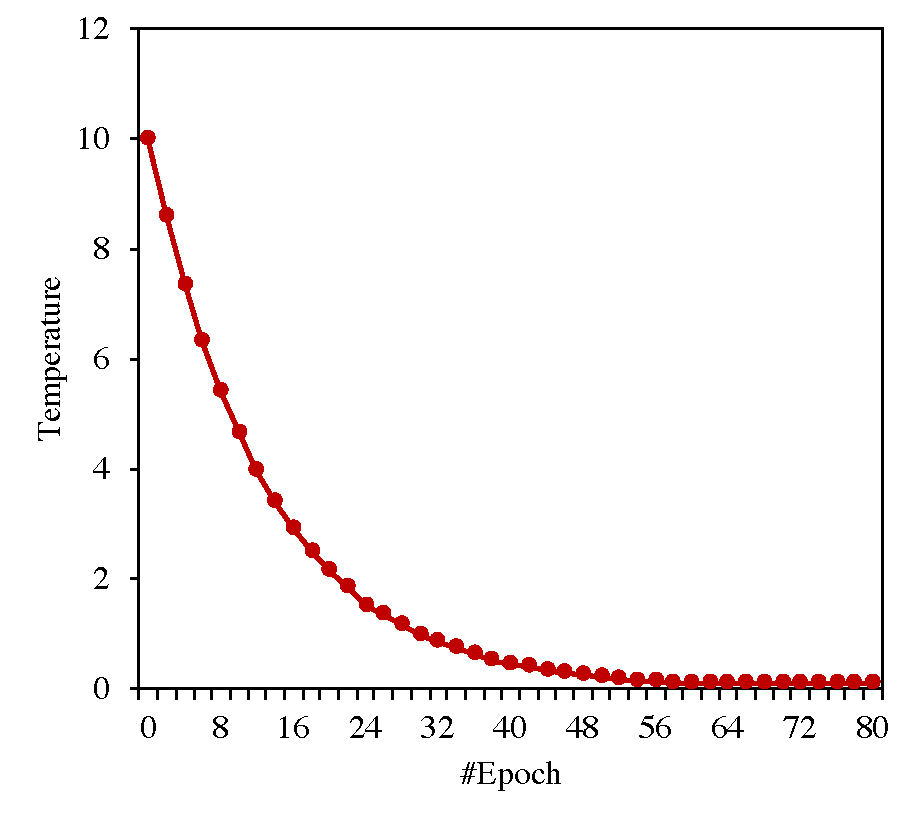
\includegraphics[scale=0.5]{fig/temp-epoch-mRNA.pdf}
    \caption{\textbf{Annealing schedules for the CoRAE.} Effect of different annealing schedules on a
concrete autoencoder trained on the mRNA dataset with $k$ = 100
selected features. If
the temperature is exponentially decayed (the annealing schedule), the feature selected layer (model) converges to informative features.}
    \label{fig:temp}
\end{figure}
\begin{figure*}[hbt]
    \centering
    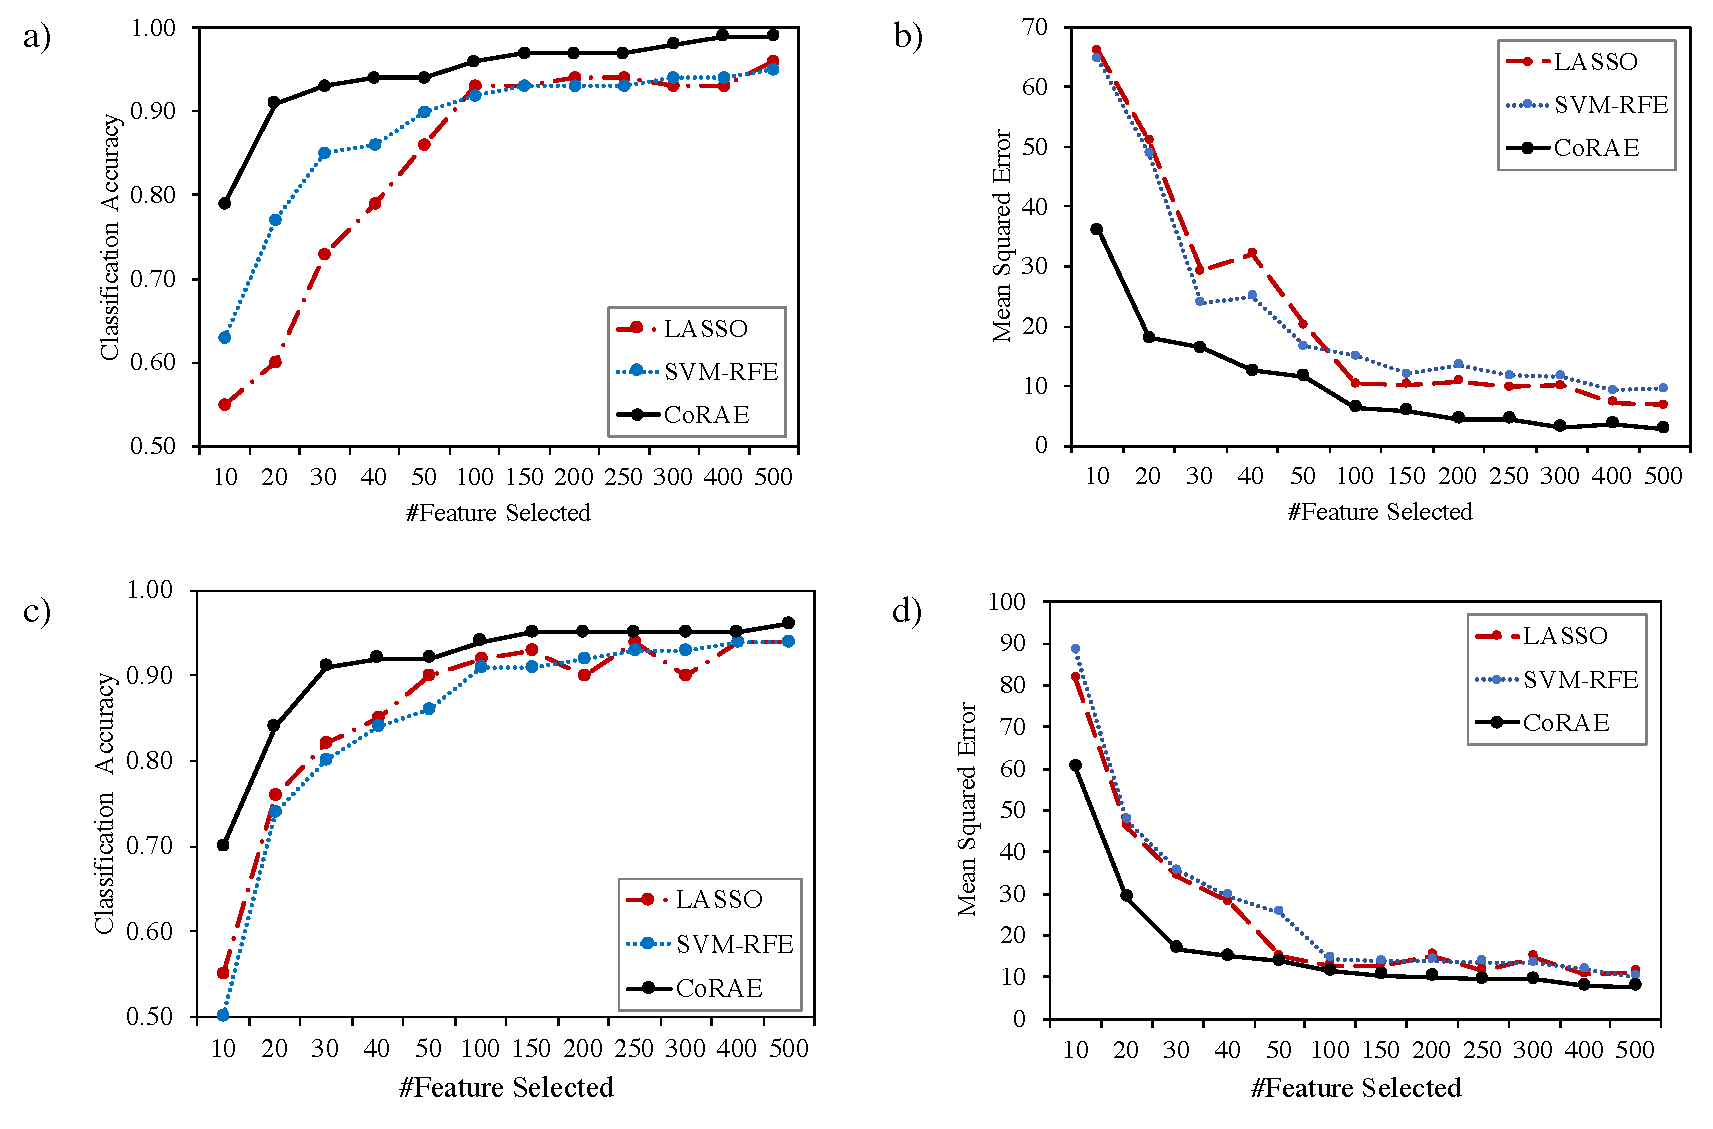
\includegraphics[scale=0.5]{fig/acc-mse.pdf}
    \caption{\textbf{Classification performance using selected RNA features.}  Comparison of CoRAE with other feature selection methods. Througout the all values of $k$ tested on both mRNA(a) and lncRNA(c) CoRAE have highest classifcation accuracy. Similarly, it shows lowest reconstruction mean squared error on both mRNA(b) and lncRNA(d)}
    \label{fig:acc-mse}
\end{figure*}
\subsection{Gene Selection, Classification, Reconstruction, and Evaluation} \label{method-details}
%\subsubsection{Feature Selection}
The encoder of the Concrete relaxation autoencoder (CoRAE) architecture is constructed with a hidden layer of $k$ nodes where $k$ being the number of gene selected. The decoder, on the other hand, is consisting of one hidden layer with 3k/2 nodes. The number of nodes in this layer is tunned in a range of [4k/7, 2k/5, 3k/2]. Adam optimizer with a learning rate of $10^-3$ is used for all the experiments. The starting temperature of the CoRAE was set to 10 and it ends at 0.01. To avoid overfitting, the dataset is split into the train and test set according to $75/25$ ratio. The training set is used to estimates the learning parameters and the test set is used for performance evaluation. To control the performance, the model is trained for the same number of epoch 100. 
Performance of CoRAE has been compared with state-of-the-art feature selection techniques such as LASSO and SVM-RFE on both mRNA and lncRNA expression datasets. In LASSO, a regularization parameter $\alpha$ decides the number of most important features. More precisely, the higher the $\alpha$, the more feature's coefficient shrinks to zero, fewer features would be selected. Recursive feature elimination is a recursive method in which less important features are eliminated in every iteration. In the recursive feature elimination technique, SVM is used as an estimator. Linear kernel with 
a regularization parameter $C=0.05$ is used. $C$ controls the tradeoff between the error and norm of the learning weights. GridSearch algorithm is used to estimate the best set of parameters for SVM. In every iteration of RFE, the number of dropped features is set to 100. 

We extract a subset of features by varying $k$ from 10 to 500. Towards fair comparison with CoRAE, the same number of genes has been selected by LASSO and SVM-RFE. Then dataset with reduced number of features (expression of selected genes) to the SVM for classifying 33 cancer types on both mRNA and lncRNA expression. Similarly, to reconstruct all the input features, we trained a linear regressor with no regularization and measure the reconstruction mean square error. 
LASSO and SVM-RFE are developed using scikit learn framwork \citep{scikit-learn} whereas CoRAE is build using Google developed Tensorflow \citep{tensorflow2015-whitepaper} based deep learning framwork Keras \citep{chollet2015keras}. Experiments are parallelized on NVIDIA Quadro K620 GPU with 384 cores and 2GB memory devices. Five different evaluation metrics have been used to record the classification and reconstruction performance such as accuracy, precision, recall, f1 score, and mean squared error (MSE). 

Accuracy is the number of correct predictions made by the model over all kinds of predictions made. True positives(TP) and True Negatives(TN) are the correct prediction. 

    \begin{equation}
        Accuracy = \frac{TP+TN}{TP+TN+FP+FN}
    \end{equation}
    Precision is the number of correct positive results divided by the number of positive results predicted by the classifier. It indicates the predicted positive portion of the samples. 
    \begin{equation}
        Precision = \frac{TP}{TP+FP}
    \end{equation}
    Recall is the number of correct positive results divided by the number of all relevant samples.
    \begin{equation}
        Recall = \frac{TP}{TP+FN}
    \end{equation}
	F1 score is a measure of a test's accuracy. It considers both the precision and the recall of the test to compute the score.
	\begin{equation}
        F1 = 2 \times \frac{Precision \times Recall}{Precision + Recall}
    \end{equation}
    Mean squared error MSE is the avarage of $(\frac{1}{n} \sum _{i=1} ^n)$ of the square of the errors $(Y_i - Y'_i)$ where $Y_i$ is a true label and $Y'_i$ is a predicted label. All performance matrices are measured on the predicted labels and true labels of independent test samples. 

Top genes can be selected based on two criteria - a) classification accuracy needs to be higher,
and b) the number of genes should be as less as possible so that biologists can conduct a wet lab experiment
easily. The capabilities of selected genes in pan-cancer classification is visually validated using unsupervised visualization technique t-SNE \citep{maaten2008visualizing}.

%Survival analysis is conducted for testing the prognostic capabilities of selected gene set. 

\begin{figure}[hbt]
    \centering
    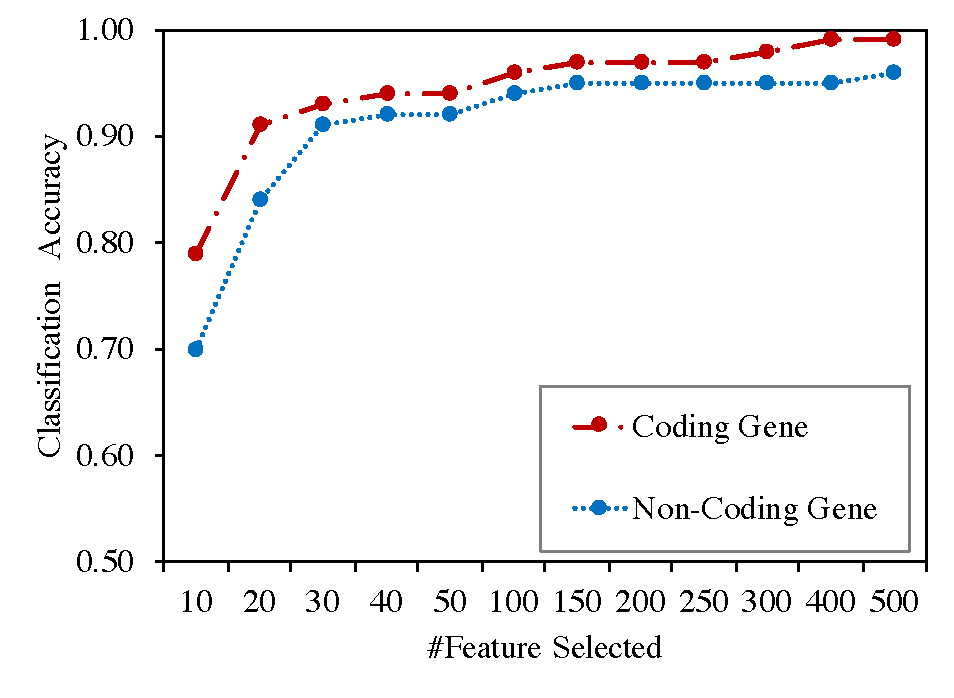
\includegraphics[scale=0.45]{fig/acc-mRNA-lncRNA.pdf}
    \caption{\textbf{Classification accuracy comparison between coding and non-coding genes expression.} Across all the $k$, mRNA expression shows slightly better classification accuracy over lncRNA expression. Here, these features has been seelcted using proposed method only.}
    \label{fig:acc-mRNA-lncRNA}
\end{figure}
\section{Results}
A series of experiements is conducted to compare the performance of CoRAE with other state-of-the-art feature selection methods such as LASSO and SVM-RFE. A range of features from 10 to 500 has been selected using all three methods, then train a linear classifier (SVM) using selected coding and non-coding gene expression of 33 cancer patients. Figure \ref{fig:acc-mse} shows the classification performance for different number of features. Across the all k, CoRAE has highest accuracy and lowest error for both mRNA and lncRNA expression. Even if the number of feature is low e.g. 10, the accuracy is almost 80\% whereas LASSO and SVM-RFE shows poor restuls for lowest number of feature. For more than 50 features, CoRAE shows more than 90\% accuracy. Also, it shows less error with less number of features compare to other methods. 
For mRNA, CoRAE starts with MSE of 38 and quickly recduced to less than 10 within top 100 features. 
The behaviour in classification is almost similar in both coding and non-coding genes. However, mRNA expression performs slightly better than lncRNA which as shown in Figure  \ref{fig:acc-mRNA-lncRNA}.

\begin{figure*}[hbt]
    \centering
    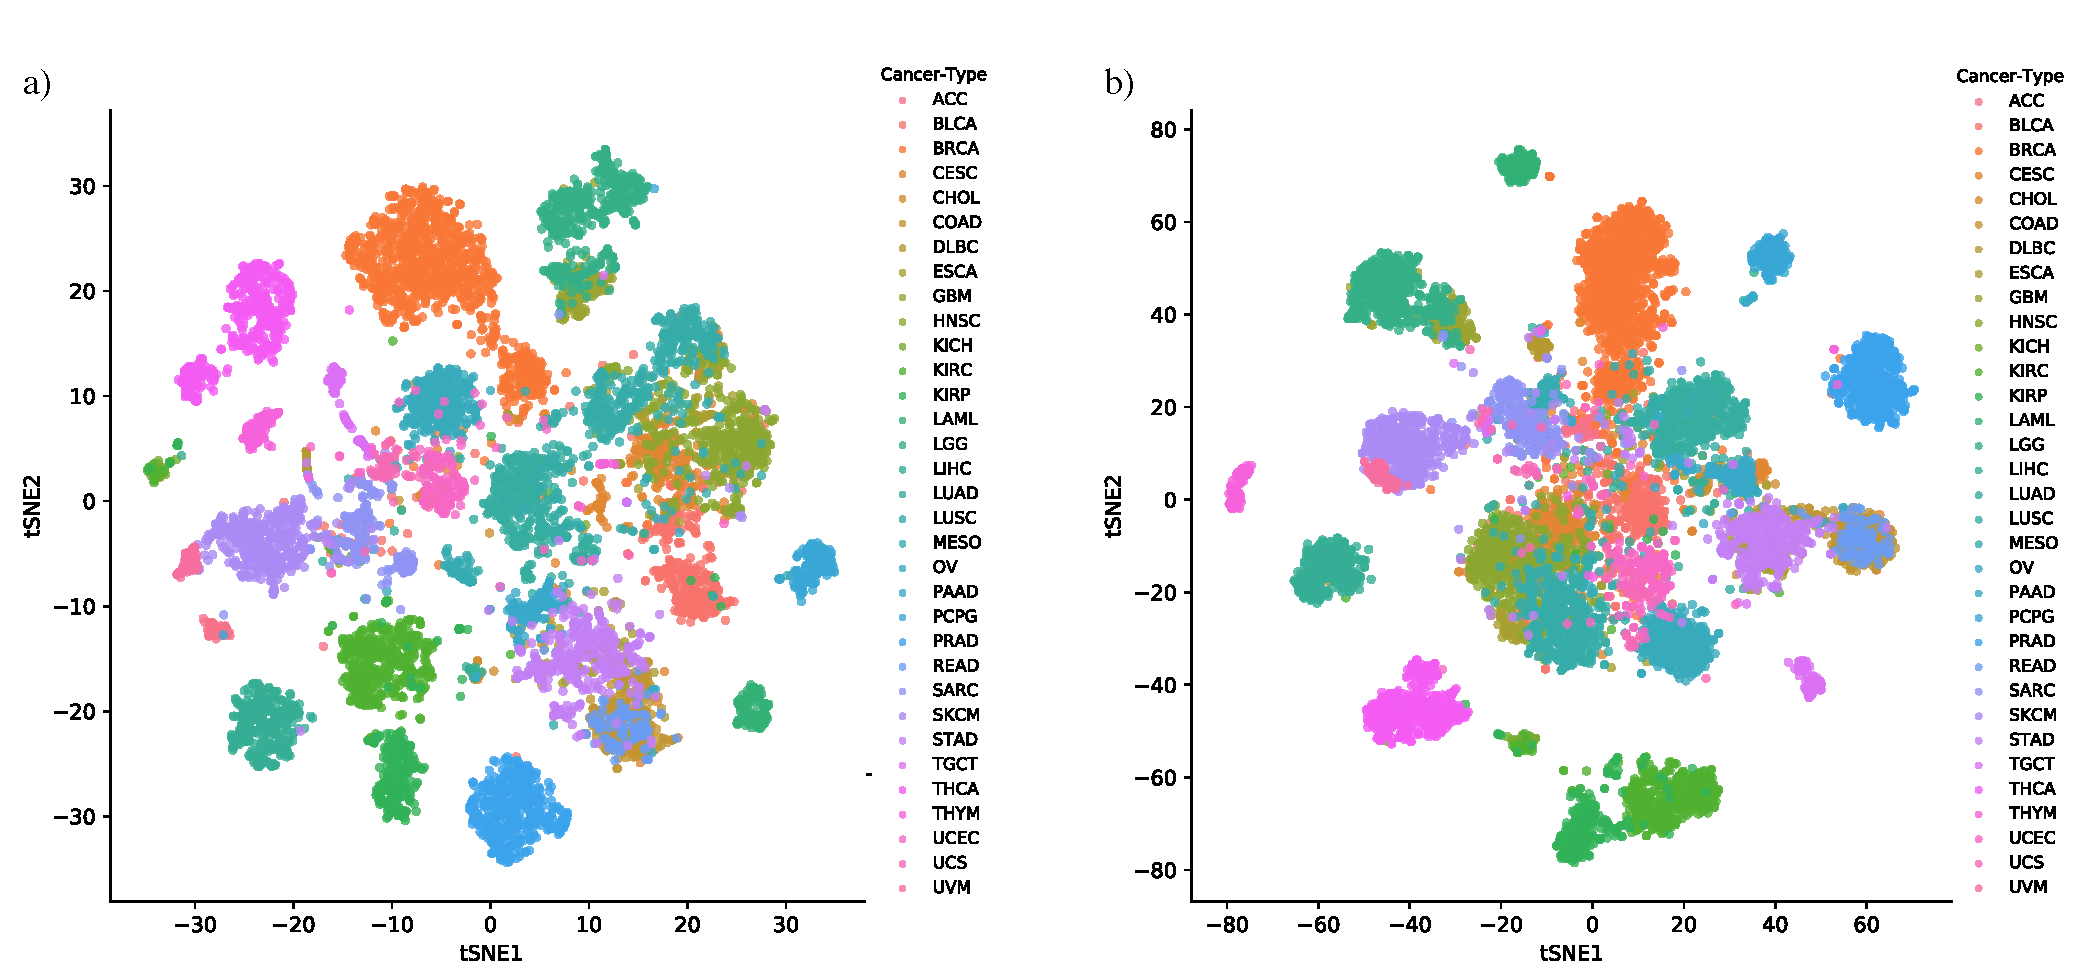
\includegraphics[scale=0.45]{fig/tSNE.pdf}
    \caption{\textbf{Visualization of 33 different cancer types using top-100 CoRAE features.} Here, we show the t-SNE representation of 33 cancer samples using selected features. Each dot represents a cancer sample and each color represents a cancer type. a) t-SNE using top 100 mRNA, b) t-SNE using top 100 lncRNA}
    \label{fig:tsne}
\end{figure*}


\subsection{Interpreting Related Features} \label{inter}
CoRAE not only able to identify important features but also allows the user to examine relevance by observing the estimated concrete parameter $\alpha^{(i)}$ for each feature. Since CoRAE selects a feature based on the value of vector $\alpha^{(i)}$, the user can check the importance of each feature and find the correlation with others.  In Figure \ref{fig:tsne}, it is visually revealed that the top 100 mRNA or lncRNA is capable of distinguishing 33 cancer types. Also, it is noticeable that the feature selected by CoRAE is carrying more information than among all other features. Thus, influential features are selected in proposed method. 
\section{Discussion}
In this research, a new differentiable feature selection method via backpropagation is proposed. In brief, the concrete relaxation autoencoder used reparameterization and concrete random variable technique to allow gradients to pass through a layer that stochastically selects discrete original input features. This randomness of the proposed method enables it to effectively search and converge to a user-defined number of original features which maximizing the objective function and minimizing the loss as discussed in section \ref{CoRAE}. The estimated parameters learned by the models can be further examined by the biologists to interpret biological relevance as discussed in section \ref{inter}. This made CoRAE distinctive from numerous competing approaches based on regularization. 

It is shown via several experiments on publicly available gene expression cancer datasets that CoRAE efficiently maximizes the classification accuracy and minimizes the reconstruction error using a selected subset of genes.  For both datasets mRNA and lncRNA gene expression, CoRAE outperformed several sophisticated feature selection techniques. This phenomena still remain and minimizes the reconstruction error when only a single hidden layer is used in the decoder.  It indicates the power of CoRAE in selecting features from a large dataset. 

Since CoRAE is built on standard autoencoder architecture, it is easily scalable to the higher number of samples or dimensions as discussed in section \ref{methods-details} where the features selected by the CoRAE outperformed the competing methods. Moreover, as CoRAE proposed in its generic form, it can be surely prolonged in several fashions. For example, unlike multiple cancer classification, important genes can be extracted during the molecular subtype classification of a single cancer dataset. Also, It allows users to integrate multi-omics data such as gene, protein, RNAseq expression, DNA methylation, copy number and so on. 
CoRAE is easy to use and it requires only a few lines of modification in implementing it in the popular machine learning algorithm. Moreover, the runtime and space complexity is similar to that of the standard autoencoder. In addition, it enhances parallelization and hardware acceleration which is an obvious demand for deep learning.  Starting and ending temperature are the only added hyperparameters used for annealing schedule. The default value used in the experiment is found well enough for the various datasets.

\section{Conclusion}
future work: we will conduct more biological validation in our extended work such as survival analysis of 33 cancer patients using selected features to measure the prognostic capabilities. Similarly, pathway analysis of selected coding and non-coding genes will be analyzed in future work as well.

\section*{Acknowledgements}


\section*{Funding}
This research is partially funded by NSF CAREER award \#1651917 (transferred to \#1901628) to AMM.

%\bibliographystyle{natbib}
%\bibliographystyle{achemnat}
%\bibliographystyle{plainnat}
%\bibliographystyle{abbrv}
\bibliographystyle{bioinformatics}
\bibliography{document}

\end{document}